% Created 2019-03-31 Sun 18:09
% Intended LaTeX compiler: pdflatex
\documentclass[12pt, aspectratio=1610]{beamer}

\usepackage{appendixnumberbeamer}
\usepackage[utf8]{inputenc}
\usepackage{ngerman}
\definecolor{sbase03}{HTML}{002B36}
\definecolor{sbase02}{HTML}{073642}
\definecolor{sbase01}{HTML}{586E75}
\definecolor{sbase00}{HTML}{657B83}
\definecolor{sbase0}{HTML}{839496}
\definecolor{sbase1}{HTML}{93A1A1}
\definecolor{sbase2}{HTML}{EEE8D5}
\definecolor{sbase3}{HTML}{FDF6E3}
\definecolor{red}{HTML}{DC322F}
\definecolor{pink}{HTML}{D33682}
\definecolor{purple}{HTML}{6C71C4}
\definecolor{blue}{HTML}{268BD2}
\definecolor{brown}{HTML}{795548}
\definecolor{cyan}{HTML}{2AA198}
\definecolor{darkgray}{HTML}{616161}
\definecolor{gray}{HTML}{9E9E9E}
\definecolor{lightgray}{HTML}{E0E0E0}
\definecolor{lime}{HTML}{CDDC39}
\definecolor{olive}{HTML}{827717}
\definecolor{orange}{HTML}{CB4B16}
\definecolor{teal}{HTML}{009688}
\definecolor{yellow}{HTML}{B58900}
\definecolor{green}{HTML}{859900}
\usepackage{listings}
\usepackage{color}
\usepackage{sourcecodepro}
\lstset{
  breaklines,
  literate={ö}{{\"o}}1
           {ä}{{\"a}}1
           {ü}{{\"u}}1,
  captionpos=b,                    % sets the caption-position to bottom
  sensitive=true,
  xleftmargin=\parindent,
  escapeinside={\%*}{*)},          % if you want to add LaTeX within your code
  basicstyle=\color{sbase00}\ttfamily,
  keywordstyle=\color{cyan},
  commentstyle=\color{sbase1},
  stringstyle=\color{blue},
  numberstyle=\color{purple},
  identifierstyle=\color{sbase00},
  showstringspaces=false,          % Removes the strange symboles where spaces are
}

\usepackage[most]{tcolorbox}
\newtcblisting{sexylisting}[2][]{
  sharp corners,
  fonttitle=\bfseries,
  colframe=gray,
  listing only,
  listing options={
    basicstyle=\color{sbase00}\ttfamily,
    keywordstyle=\color{cyan},
    commentstyle=\color{sbase1},
    stringstyle=\color{blue},
    numberstyle=\color{purple},
    identifierstyle=\color{sbase00},
    language=C,
  },
  title=\thetcbcounter #2, #1
}
\useoutertheme{sidebar}
\usetheme{metropolis}
\author{Andreas Zweili}
\date{\today}
\title{Präsentation Diplomarbeit}
\hypersetup{
 pdfauthor={Andreas Zweili},
 pdftitle={Präsentation Diplomarbeit},
 pdfkeywords={},
 pdfsubject={},
 pdfcreator={Emacs 26.1 (Org mode 9.2.2)},
 pdflang={Germanb}}
\begin{document}

\maketitle\newpage
\begin{frame}{Inhalt}
\tableofcontents
\end{frame}


\section{Einführung}
\label{sec:orgdacebc4}
\begin{frame}[label={sec:org57eb7f2}]{Einführung}
\begin{itemize}
\item <2-> Das Kommandozeilen Programm "`BorgBackup"' mittels einer grafischen
Oberfläche für normale Benutzer zugänglich machen
\item <3-> Evaluation der benötigten Technologien
\item <4-> Programmieren der Basis-Funktionen
\item <5-> Die Grundlage für ein Open-Source Projekt schaffen
\end{itemize}
\end{frame}

\begin{frame}[label={sec:org9b4cea2}]{Einführung}
\begin{columns}
\begin{column}{0.5\columnwidth}
\alert{Inspiration}
\begin{itemize}
\item <2-> Fehlende Backups im Umfeld
\item <3-> Fehlendes Know-How im Umfeld
\item <4-> Software "`Back in Time"'
\end{itemize}
\end{column}

\begin{column}{0.5\columnwidth}
\begin{center}

\includegraphics[width=.9\linewidth]{pictures/inspiration.png}
\end{center}
\end{column}
\end{columns}
\end{frame}

\begin{frame}[label={sec:org0bb2172}]{Einführung}
\begin{columns}
\begin{column}{0.5\columnwidth}
\alert{Wieso BorgBackup?}
\begin{itemize}
\item <2-> Open-Source Software
\item <3-> Ist cross-plattform fähig
\item <4-> Blockbasierte Deduplikation
\end{itemize}
\end{column}

\begin{column}{0.5\columnwidth}
\begin{center}

\includegraphics[width=.9\linewidth]{pictures/borg.jpeg}
\end{center}
\end{column}
\end{columns}
\end{frame}

\begin{frame}[label={sec:orgdce3104}]{Einführung}
\alert{Blockbasierte Deduplikation}

\begin{center}
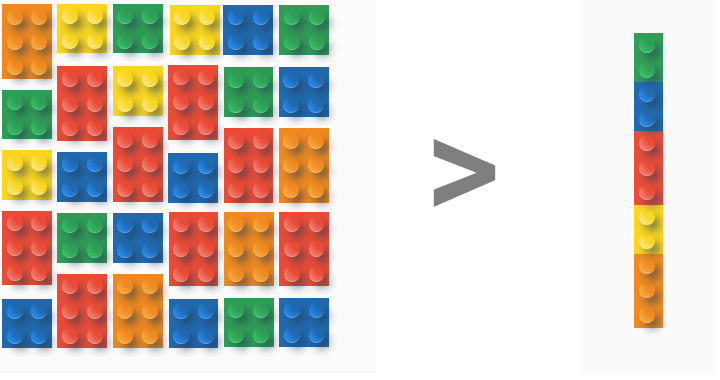
\includegraphics[width=.9\linewidth]{pictures/deduplication.png}
\end{center}
\end{frame}


\section{Projekt Management}
\label{sec:orga12f2d6}
\begin{frame}[label={sec:org9df78e5}]{Projekt Mangement}
\begin{columns}
\begin{column}{0.5\columnwidth}
\alert{Wasserfallmodell}
\begin{itemize}
\item <2-> Funktioniert gut für Einzelpersonen
\item <3-> Phasenbasiertes Modell
\end{itemize}
\end{column}

\begin{column}{0.5\columnwidth}
\begin{center}
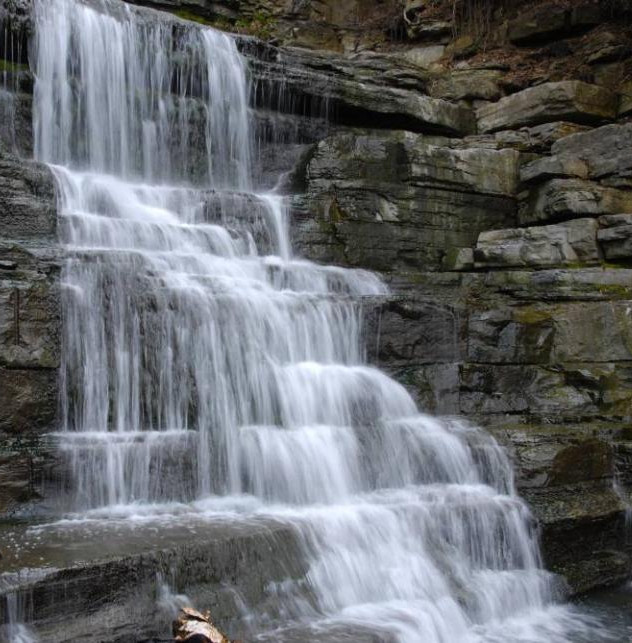
\includegraphics[width=.8\linewidth]{pictures/waterfall_stairs.jpg}
\end{center}
\end{column}
\end{columns}
\end{frame}

\begin{frame}[label={sec:orgb561a63}]{Projekt Management}
\begin{columns}
\begin{column}{0.50\columnwidth}
\alert{Ist-Risiko nicht funktionaler Backups}
\begin{enumerate}
\item <2-> Falsche Nutzung einer Kommandozeilen Applikation
\item <3-> Backups ohne Verschlüsselung
\item <4-> Falscher Speicherort
\item <5-> Versehentliche Löschung
\item <6-> User vergisst Backups zu machen
\end{enumerate}
\end{column}

\begin{column}{0.45\columnwidth}
\begin{center}
\includegraphics<2>[width=\linewidth]{pictures/istrisiko1.pdf}%
\includegraphics<3>[width=\linewidth]{pictures/istrisiko2.pdf}%
\includegraphics<4>[width=\linewidth]{pictures/istrisiko3.pdf}%
\includegraphics<5>[width=\linewidth]{pictures/istrisiko4.pdf}%
\includegraphics<6>[width=\linewidth]{pictures/istrisiko.pdf}%
\end{center}
\end{column}
\end{columns}
\end{frame}

\begin{frame}[label={sec:org43ac6cb}]{Projekt Mangement}
\begin{columns}
\begin{column}{0.45\columnwidth}
\alert{Ist-Risiko}
\begin{center}
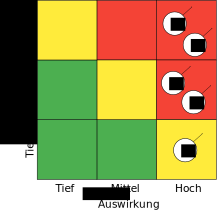
\includegraphics[width=\linewidth]{pictures/istrisiko.pdf}%
\end{center}
\end{column}

\begin{column}{0.45\columnwidth}
\onslide<2->\alert{Soll-Risiko}
\begin{center}
\includegraphics<2->[width=\linewidth]{pictures/sollrisiko.pdf}%
\end{center}
\end{column}
\end{columns}
\end{frame}

\begin{frame}[label={sec:org774531d}]{Projekt Mangement}
\alert{Controlling}

\begin{center}
\begin{tabular}{lll}
\textbf{Phase} & \textbf{Gesch. Aufwand} & \textbf{Effekt. Aufwand}\\
\hline
Initialisierung & 22h & 20.3h\\
\hline
Analyse & 47h & 41.6h\\
\hline
Konzept & 34h & 35.1h\\
\hline
Realisierung & 172h & 149.3h\\
\hline
Abschluss und Meetings & 43h & 42.07h\\
\hline
\alert{Total} & 318h & 288.37h\\
\end{tabular}

\end{center}
\end{frame}

\section{Lösungsvarianten}
\label{sec:org735a602}
\begin{frame}[label={sec:org5e5a1cd}]{Lösungsvarianten}
\alert{Kriterien}
\begin{itemize}
\item <2-> Cross-plattform kompatibel
\item <3-> Freie Software
\item <4-> Vorkenntnisse
\item <5-> Integriert sich gut ins System
\item <6-> Ohne spezielle Tools nutzbar
\end{itemize}
\end{frame}

\begin{frame}[label={sec:org28f8125}]{Lösungsvarianten}
\begin{columns}
\begin{column}{0.3\columnwidth}
\alert{Backend}
\begin{itemize}
\item <2-> C\#
\item <3-> Python
\item <4-> C++
\end{itemize}
\end{column}

\begin{column}{0.5\columnwidth}
\begin{center}
\includegraphics<2>[width=\linewidth]{pictures/backend1.png}%
\includegraphics<3>[width=\linewidth]{pictures/backend2.png}%
\includegraphics<4>[width=\linewidth]{pictures/backend3.png}%
\end{center}
\end{column}
\end{columns}
\end{frame}

\begin{frame}[label={sec:org1a107a3}]{Lösungsvarianten}
\begin{columns}
\begin{column}{0.3\columnwidth}
\alert{Frontend}
\begin{itemize}
\item <2-> Qt
\item <3-> Gtk
\item <4-> Electron
\end{itemize}
\end{column}

\begin{column}{0.5\columnwidth}
\begin{center}
\includegraphics<2>[width=.9\linewidth]{pictures/frontend1.png}%
\includegraphics<3>[width=.9\linewidth]{pictures/frontend2.png}%
\includegraphics<4>[width=.9\linewidth]{pictures/frontend3.png}%
\end{center}
\end{column}
\end{columns}
\end{frame}

\begin{frame}[label={sec:orgc8f3f46}]{Lösungsvarianten}
\alert{Resultat}

\begin{center}

\includegraphics[height=.5\textheight]{pictures/pyqt.png}
\end{center}
\end{frame}

\section{Umsetzung}
\label{sec:org34c5953}
\begin{frame}[label={sec:orgc77a9ca}]{Umsetzung}
\begin{columns}
\begin{column}{0.3\columnwidth}
\alert{Werkzeuge}

\begin{itemize}
\item Gnome Planner
\item Emacs
\item Git
\item Qt-Designer
\item Inkscape
\item Draw.io
\item Virtualbox
\end{itemize}
\end{column}

\begin{column}{0.5\columnwidth}
\begin{center}

\includegraphics[width=.9\linewidth]{pictures/tools7.png}%
\end{center}
\end{column}
\end{columns}
\end{frame}

\begin{frame}[label={sec:org55d0100}]{Umsetzung}
\alert{Finales Produkt}

\begin{center}
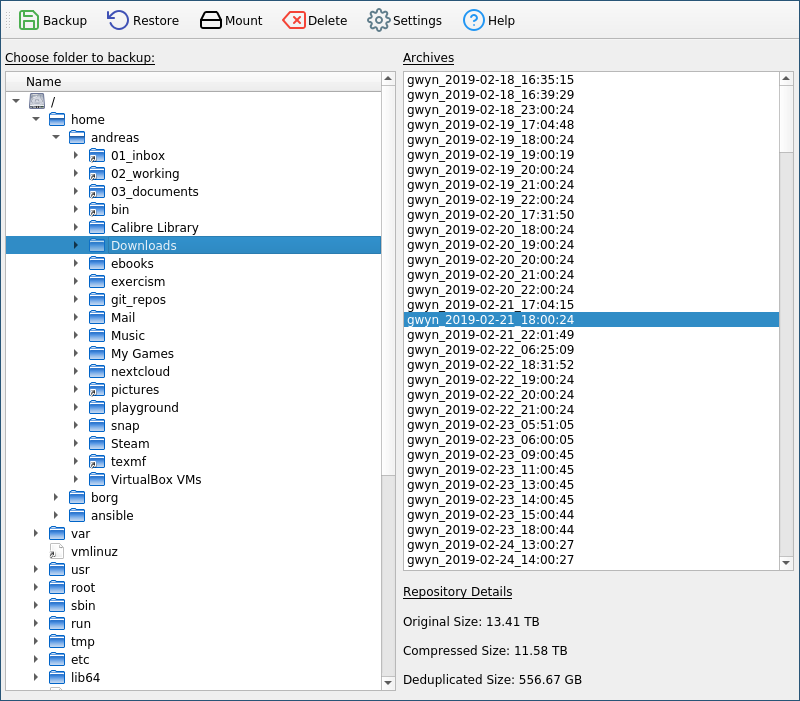
\includegraphics[height=.8\textheight]{pictures/borgqt1.png}%
\end{center}
\end{frame}

\begin{frame}[label={sec:org0493ab9}]{Umsetzung}
\alert{Finales Produkt}

\begin{center}
\frame{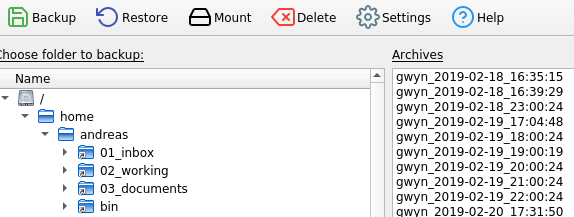
\includegraphics[width=\textwidth]{pictures/borgqt5.png}}%
\end{center}
\end{frame}

\begin{frame}[label={sec:org637fa6c}]{Umsetzung}
\alert{Finales Produkt}

\begin{center}
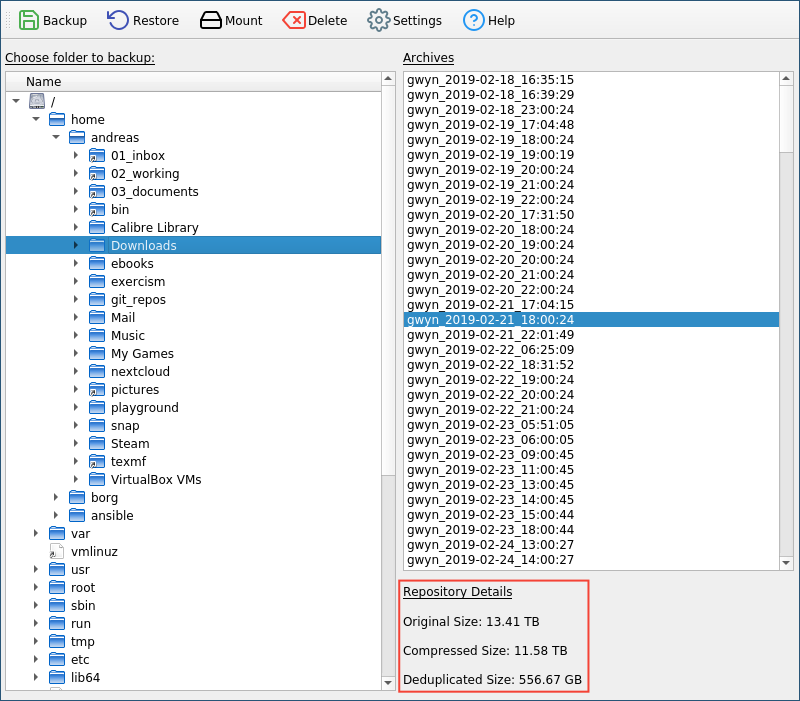
\includegraphics[height=.8\textheight]{pictures/borgqt2.png}%
\end{center}
\end{frame}

\begin{frame}[label={sec:org1b99856}]{Umsetzung}
\begin{center}
\begin{tabular}{ll}
\textbf{Speicherverbrauch} & \\
\hline
Reale Grösse & 13.41 TB\\
Deduplizierte Grösse & 556.67 GB\\
\end{tabular}

\end{center}

\begin{center}
24x weniger Speicherverbrauch
\end{center}
\end{frame}

\begin{frame}[label={sec:org5aa0508}]{Umsetzung}
\begin{columns}
\begin{column}{0.45\columnwidth}
\alert{Soll-Risiko}
\begin{center}
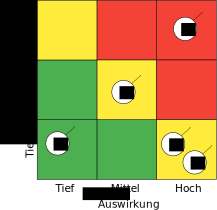
\includegraphics[width=\linewidth]{pictures/sollrisiko_grey.pdf}%
\end{center}
\end{column}

\begin{column}{0.45\columnwidth}
\onslide<2->\alert{Neues Ist-Risiko}
\begin{center}
\includegraphics<2->[width=\linewidth]{pictures/ist_risiko_neu.pdf}%
\end{center}
\end{column}
\end{columns}
\end{frame}

\section{Abschluss}
\label{sec:orgdb433f2}
\begin{frame}[label={sec:org33a667a}]{Abschluss}
\alert{Fazit}
\begin{itemize}
\item <2-> Die Arbeit war sehr interessant und zeitintensiv
\item <3-> Ganttcharts können sehr hilfreich sein um den Fokus zu halten
\item <4-> Automatisierte Tests sind ein Must-have für Entwickler, sind jedoch zeitintensiv
\end{itemize}
\end{frame}

\begin{frame}[label={sec:org91d75ee}]{}
\alert{\huge{Fragen?}}
\end{frame}
\begin{frame}[label={sec:org1172673}]{}
\alert{\huge{Vielen Dank für die Aufmerksamkeit!}}
\end{frame}
\end{document}